\chapter{Introduction}
Rephotography denotes the retrieval of the precise viewpoint used for taking a
--- possibly historic --- photograph and capturing another image from the same
spot, ideally with the same camera parameters. This allows for
documentation and visualisation of changes which the scene has undergone between
the two or more captures.  For instance, one can present progress of
construction, restoration efforts or changes in the surroundings in a visually
striking manner, for instance by blending the photographs together. 
Figures \autoref{fig1} and \autoref{fig2} show examples.

\begin{figure}
   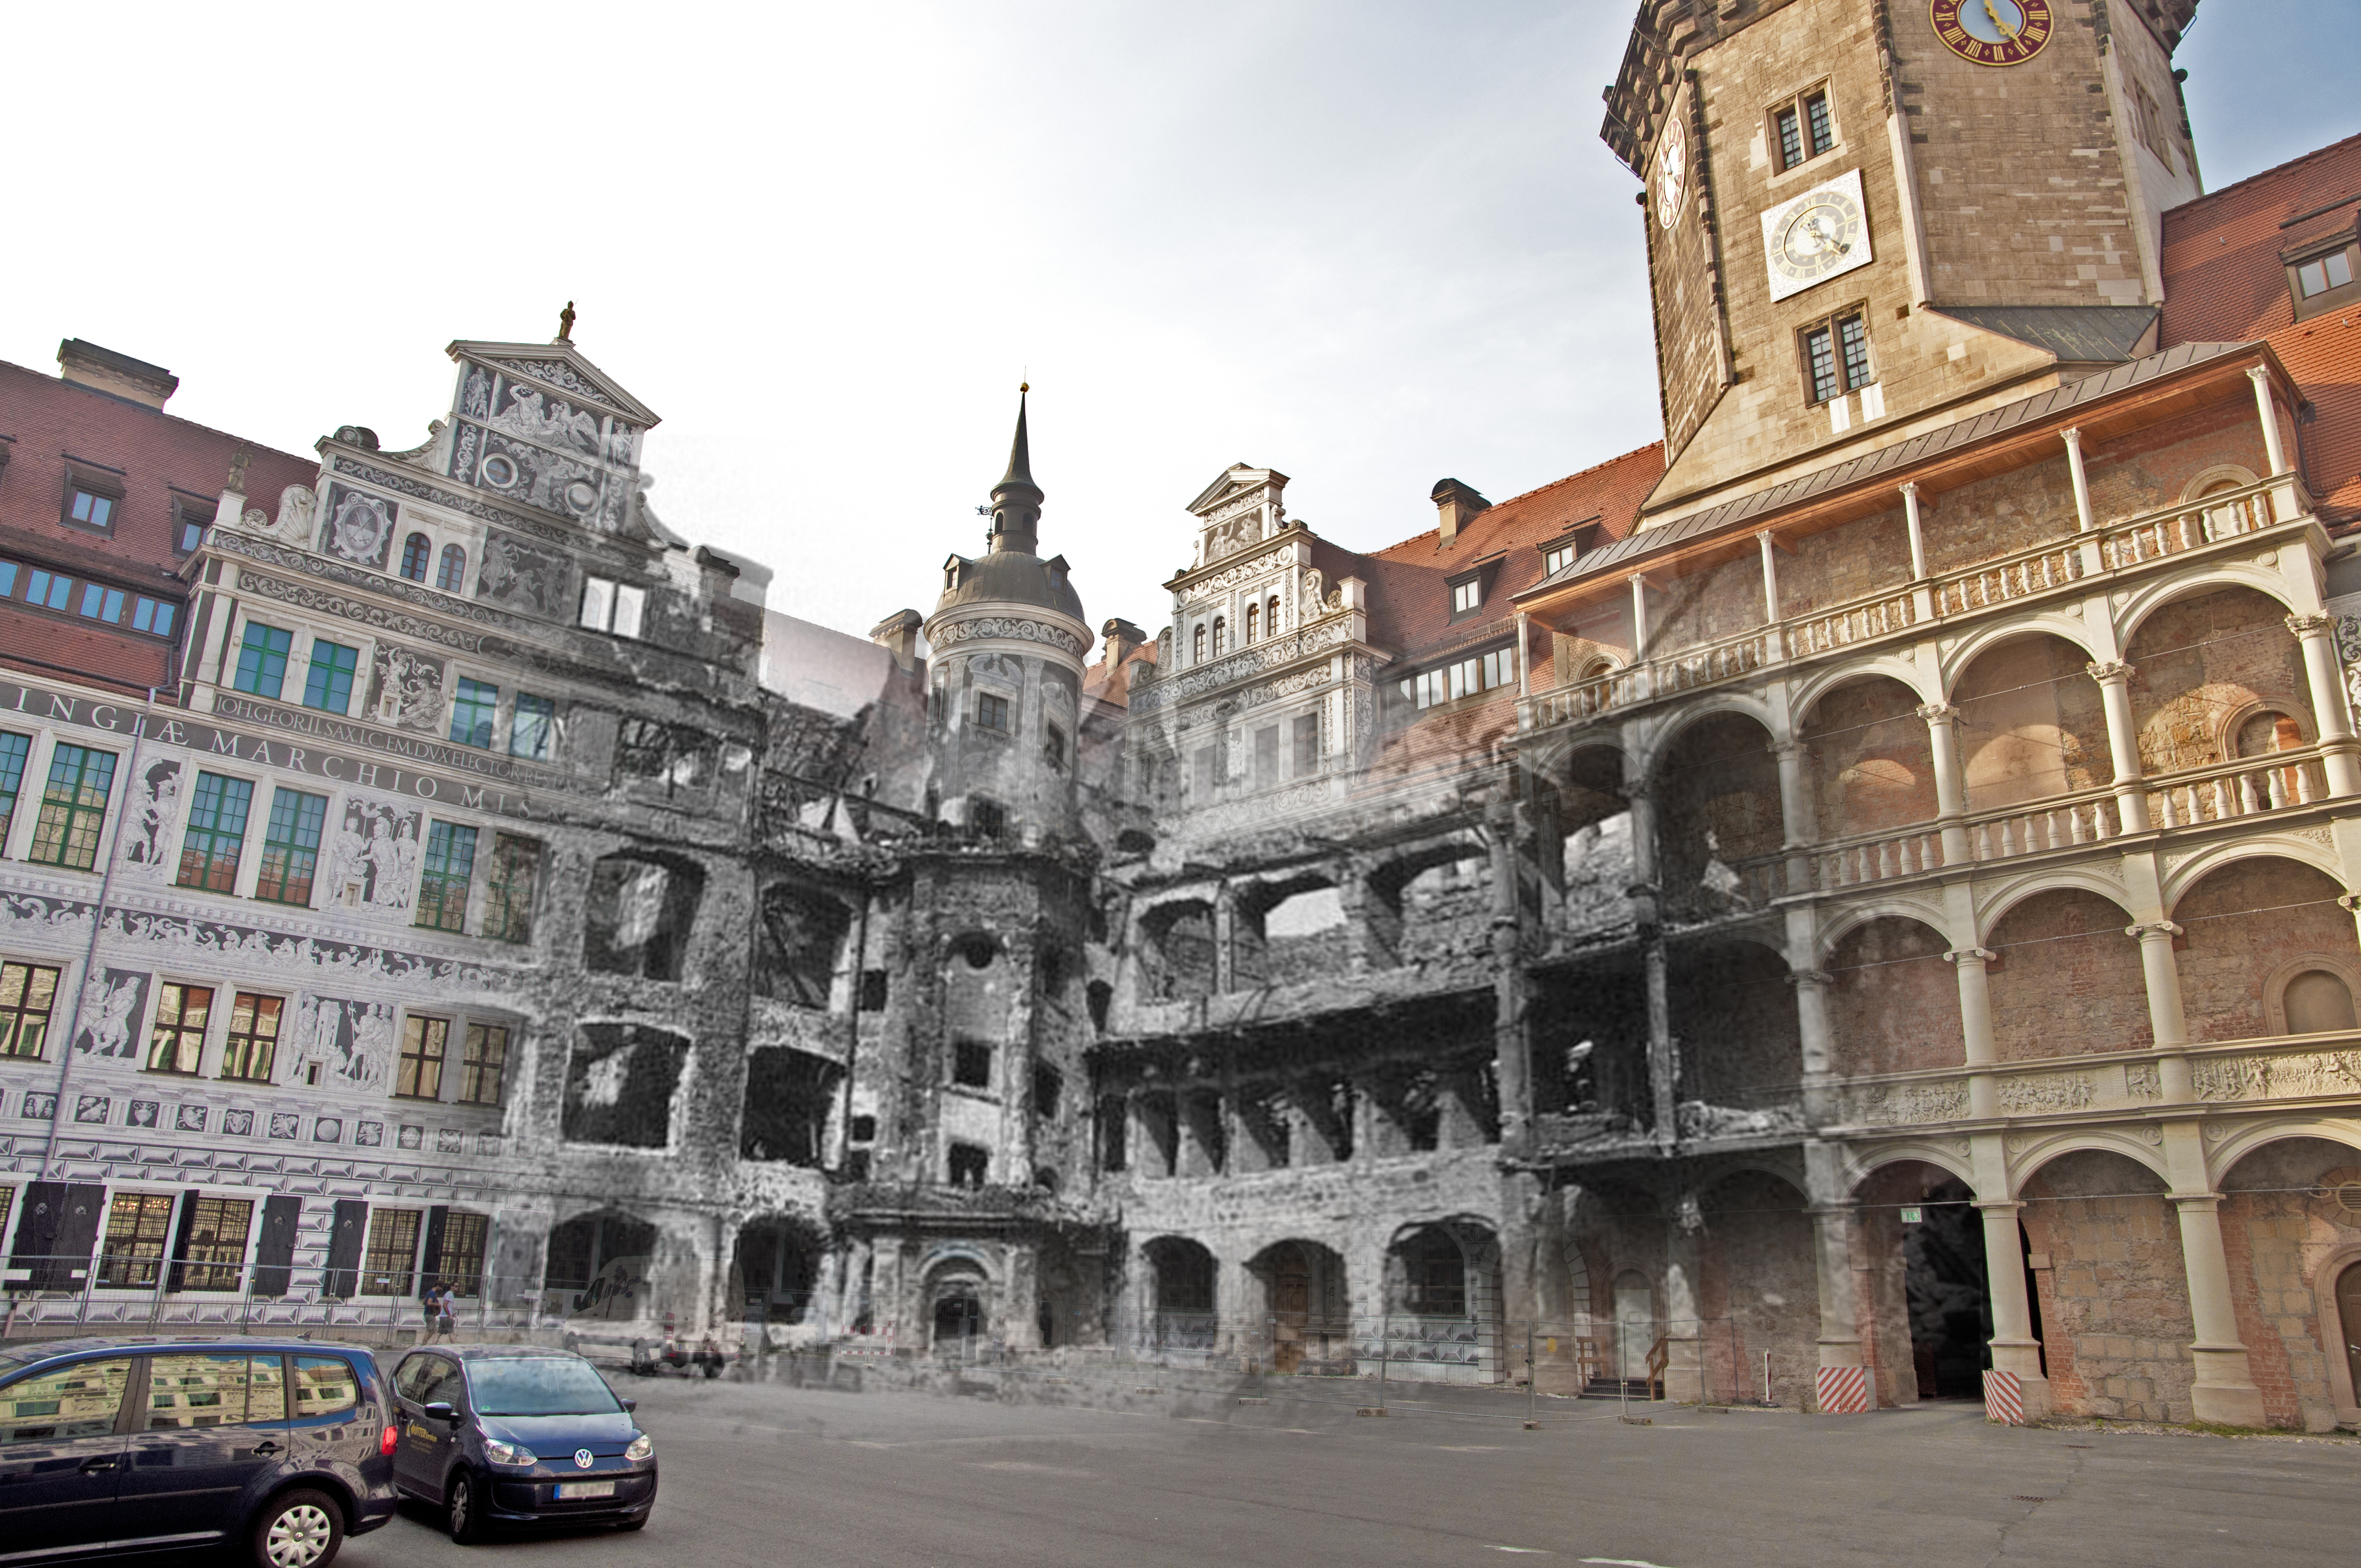
\includegraphics[width=\textwidth]{gfx/1945_2014_Residenzschloss.jpg}
   \caption{Residenzschloss in Dresden, destroyed during World War II,
   \textcopyright\ Sergey Larenkov, printed with permission}
   \label{fig1}
\end{figure}

\begin{figure}
   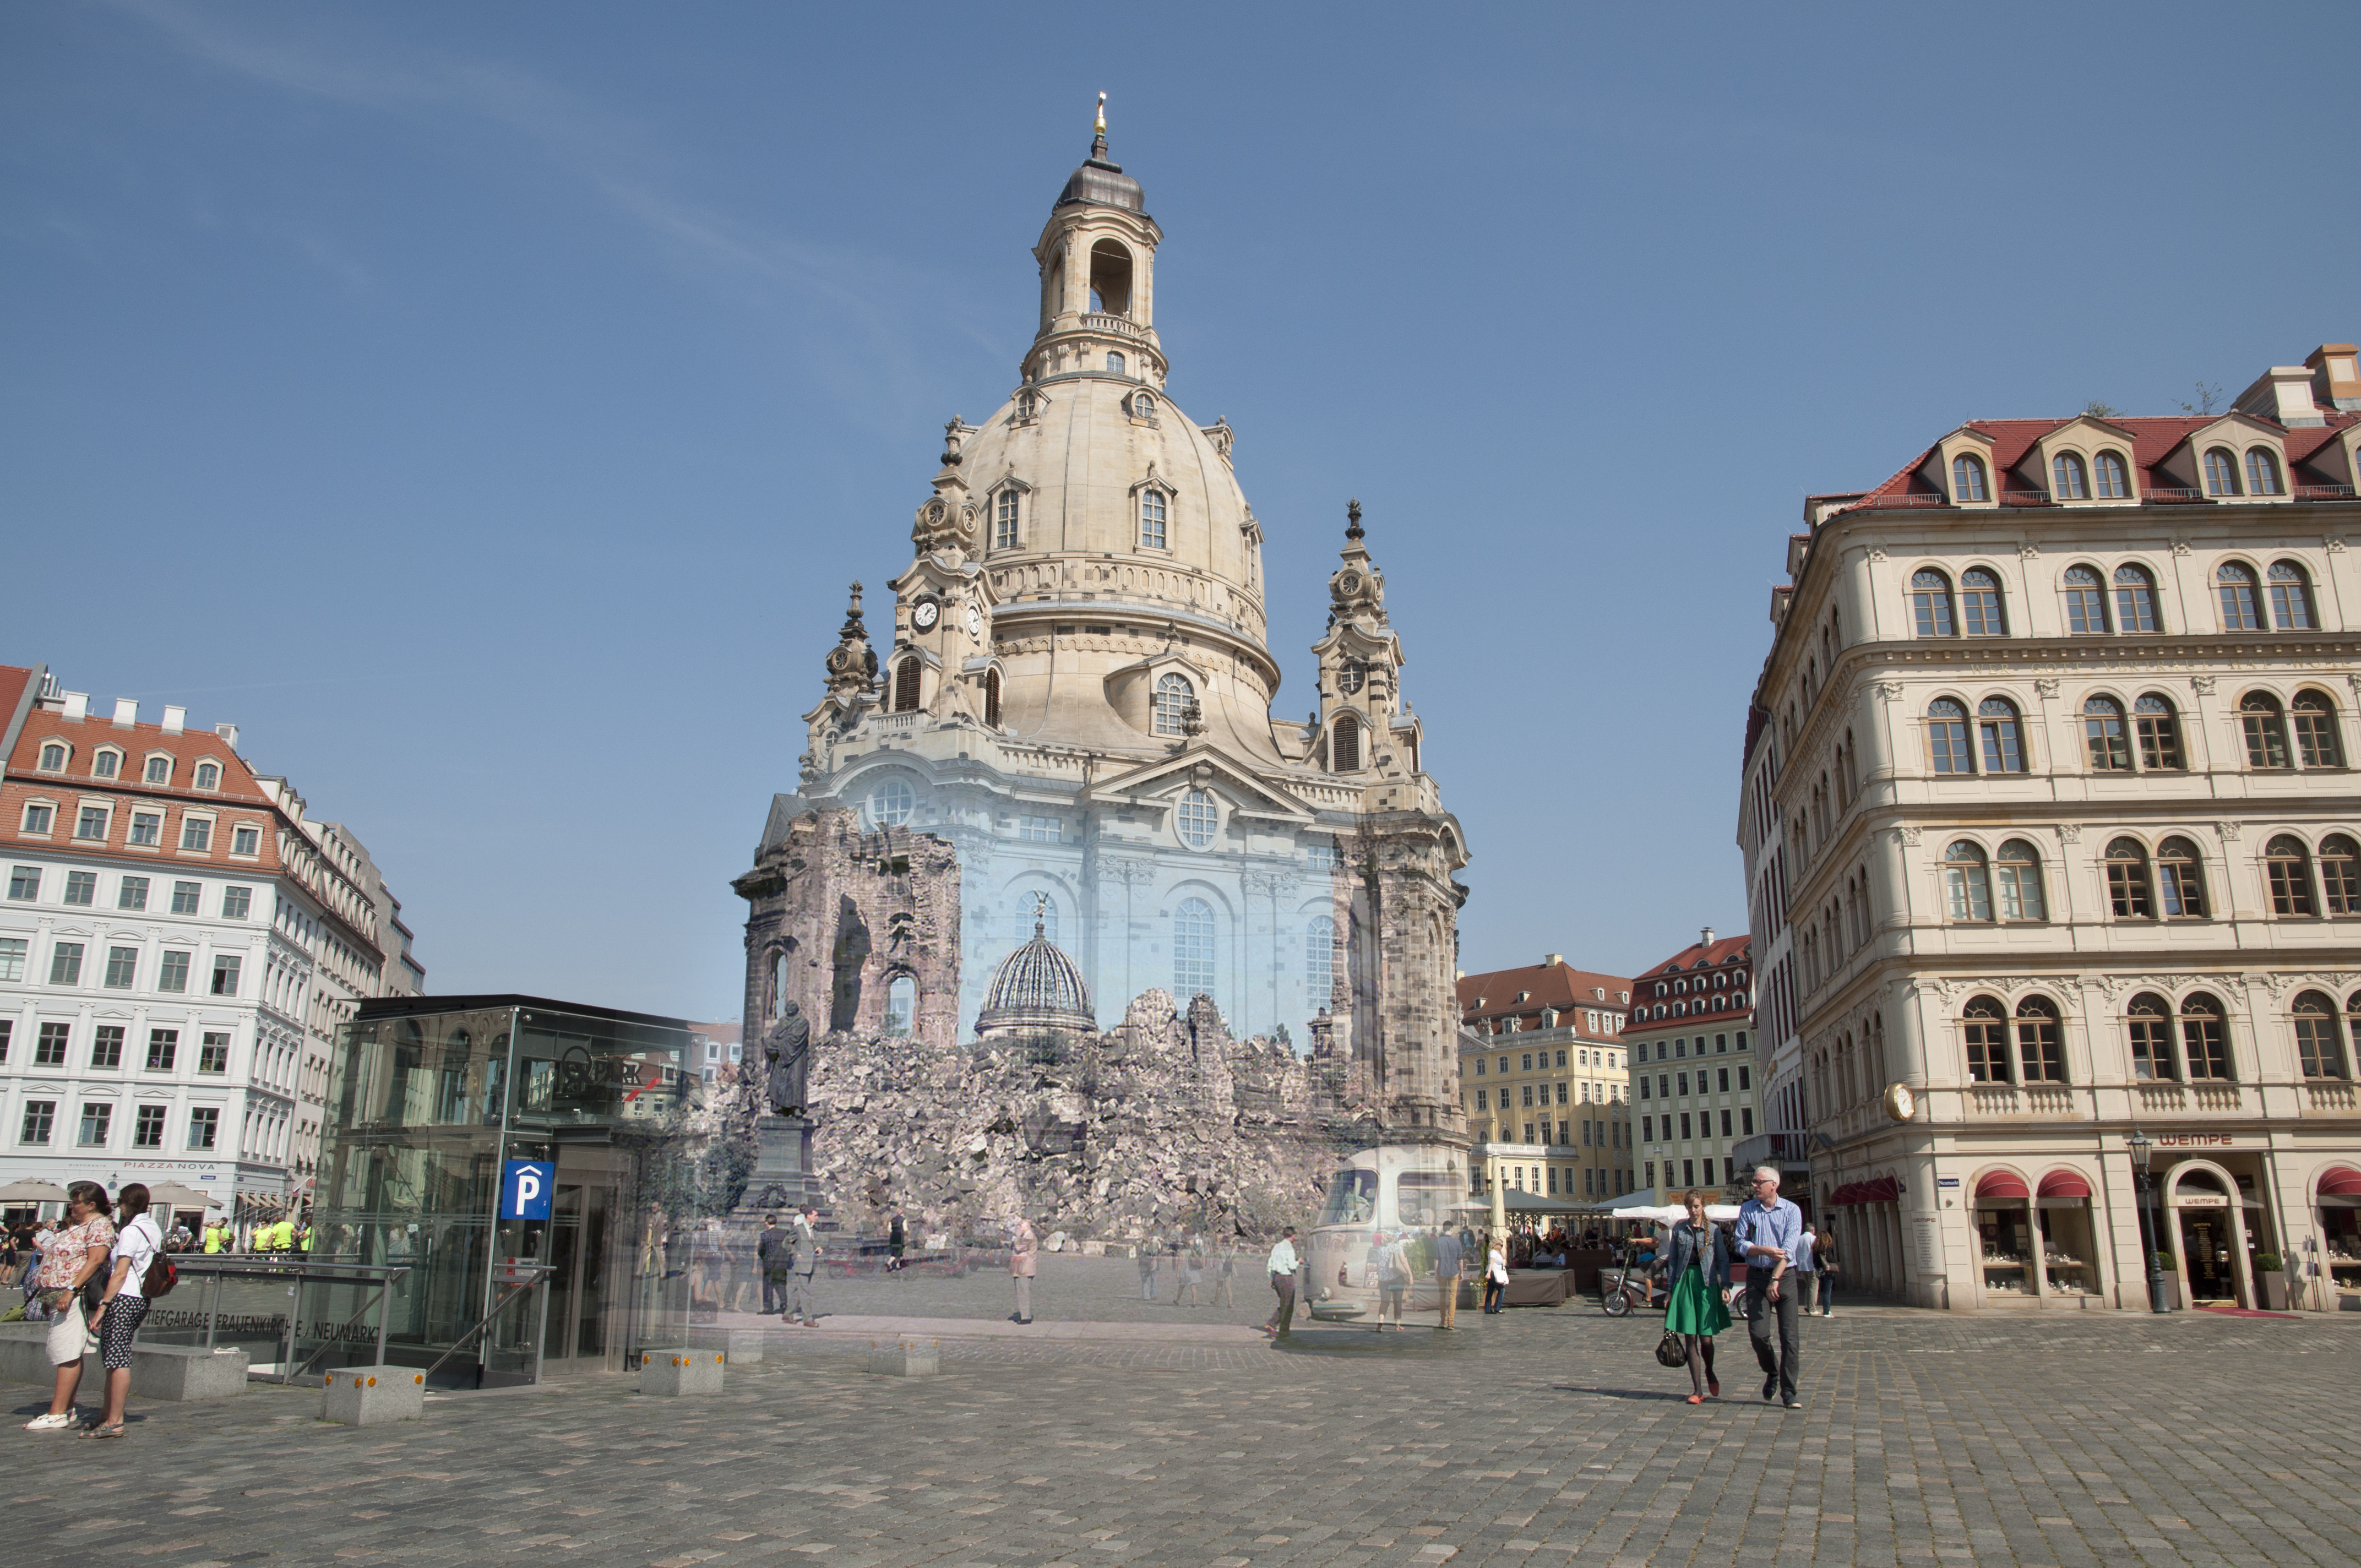
\includegraphics[width=\textwidth]{gfx/1950_2014_Frauenkirche.jpg}
   \caption{Frauenkirche in Dresden, destroyed during World War II,
   \textcopyright\ Sergey Larenkov, printed with permissio}
   \label{fig2}
\end{figure}

When done manually, the photographer must attempt to find the original viewpoint 
usually by visual inspection of the original image and trying to match the
current camera parameters --- camera position, camera rotation, focal length,
possibly principal point --- to the original.
The procedure is often carried out by placing the camera on a tripod and
comparing a printout of the original image with what can be seen through the
viewfinder or the camera screen. The number of parameters to match as well as
the difficulty to estimate them purely from comparing images makes the process
error-prone and tedious.

The advancement of mobile phones or tablet computers with integrated cameras and
larger screens
presents the opportunity to develop applications which can assist in this
endeavour, which is impossible on digital cameras due to their closed
infrastructure not permitting running user programs.
